\section{Komunikacja między elementami oprogramowania}
\label{sec:komunikacja}

Hybrydowa struktura aplikacji wymusza dokładne zdefiniowanie schematów komunikacyjnych między oboma jej poziomami.
Poniżej znajduje się podsumowanie wartości wysyłanych przez oba poziomy.

\begin{enumerate} 
    \item Część obliczeniowa wysyła:
    \begin{enumerate}
        \item wartości końcowe poziomów w zbiornikach (będące stanem docelowym w zadaniu czasooptymalnym oraz punktem linearyzacji modelu służącym do wyliczenia nastaw regulatora liniowo-kwadratowego),
        \item dla sterowania czasooptymalnego:
        \begin{enumerate}
            \item czasy przełączeń,
            \item wartość początkową sterowania czasooptymalnego,
            \item wartość ,,drugorzędną'' tego sterowania (założono, że niższy poziom aplikacji nie musi znać ograniczeń nałożonych na sterowanie),
            \item czas optymalny;
        \end{enumerate}
        \item dla sterowania liniowo-kwadratowego:
        \begin{enumerate}
            \item wektor K współczynników regulatora,
            \item sterowanie ustalone, od którego są liczone odchyłki.
        \end{enumerate}
    \end{enumerate}
    \item Część sterowania bezpośredniego wysyła:
    \begin{enumerate}
        \item aktualne poziomy wody w zbiornikach,
        \item aktualną wartość sterowania.
    \end{enumerate}
\end{enumerate}

Poniżej znajduje się ich lista wyszczególnionych 3 możliwych akcji zachodzących w systemie. Zilustrowano je odpowiednimi (aczkolwiek uproszczonymi do poziomu ogólnej specyfikacji) diagramami sekwencji według konwencji UML (ang. \emph{Unified Modelling Language}). Wyszczególniono na nich użytkownika, część obliczeniową i sterującą oraz oprogramowanie optymalizacyjne, aby zaznaczyć, że jest ono de facto osobnym elementem, zewnętrznym i niestanowiącym części aplikacji będącej przedmiotem niniejszej pracy.

\begin{enumerate}
    \item Akcja obliczania sterowania czasooptymalnego (przedstawiona na rys. \ref{fig:comm-toc}).
    \item Akcja obliczania sterowania liniowo-kwadratowego (pokazana na rys. \ref{fig:comm-lqr}).
    \item Akcja wysłania obliczonych sterowań między poziomami aplikacji (zaprezentowana na rys. \ref{fig:comm-send} zawierającym pozostałe akcje w uproszczonej formie).
\end{enumerate}

Zdecydowano, że protokołem przesyłu danych między poziomami aplikacji będzie TCP (ang. \emph{Transmission Control Protocol}). Jest to zdecydowanie najpopularniejszy sposób przesyłu danych w sieci Internet między dwoma urządzeniami, z których jedno jest serwerem, a drugie klientem. Ze względu na to, że wyższy poziom aplikacji dostarcza większej ilości danych, zdecydowano, że to właśnie on będzie działał jako serwer TCP.

\begin{figure}[hpt]
    \centering
    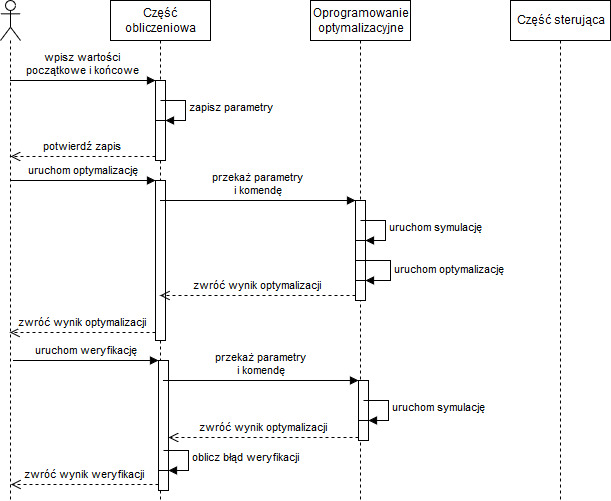
\includegraphics[width=\textwidth]{Grafika/communication-toc}
    \caption{Diagram sekwencji ilustrujący akcję obliczenia sterowania czasooptymalnego. Źródło: własne.}\label{fig:comm-toc}
\end{figure}

\begin{figure}[hpt]
    \centering
    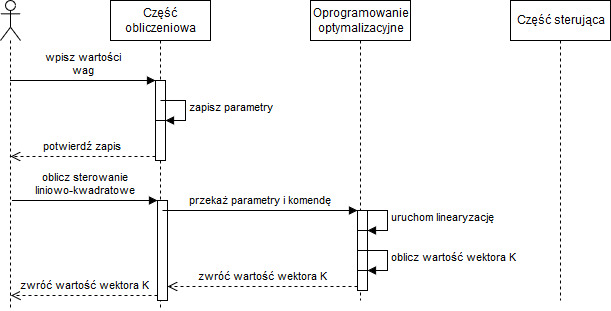
\includegraphics[width=\textwidth]{Grafika/communication-lqr}
    \caption{Diagram sekwencji ilustrujący akcję obliczenia sterowania liniowo-kwadratowego. Źródło: własne.}\label{fig:comm-lqr}
\end{figure}

\begin{figure}[hpt]
    \centering
    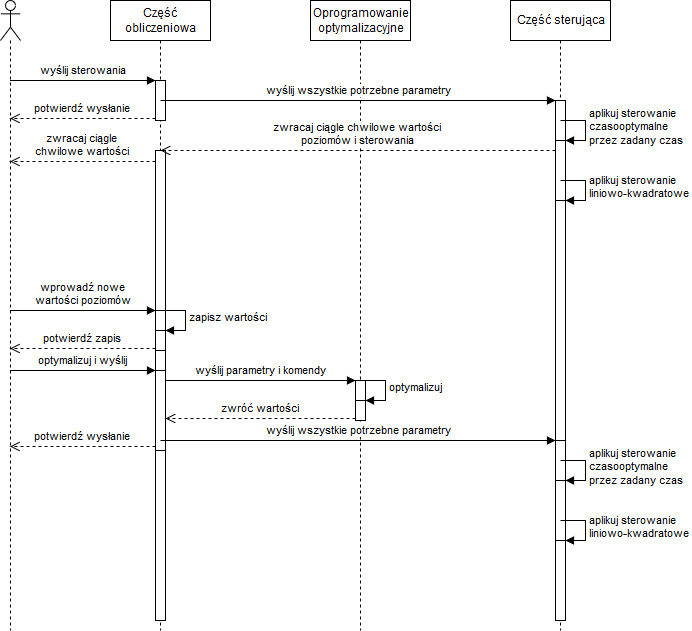
\includegraphics[width=\textwidth]{Grafika/communication-between-levels}
    \caption{Diagram sekwencji ilustrujący akcję wysyłania sterowań. Źródło: własne.}\label{fig:comm-send}
\end{figure}
